\section*{Лекция 1 (17.02.2022)}
\section{Интегральное исчисление функций}
\subsection{Первообразная и неопределенный интеграл}

\begin{definition}
    $f : (a, b) \rightarrow \R, F : (a, b) \rightarrow \R$, $F$ -- первообразная $f$ на $(a, b)$ если $F' = f$
\end{definition}


\begin{theorem}
    $f, F : (a, b) \rightarrow \R$, $F$ -- первообразная $f$ 
    \begin{enumerate}
    \item $\Rightarrow F + c$ - первообразная $f$
    \item $G : (a,b)$ - первообразная $f \Rightarrow F - G = const$ 
    \end{enumerate}
\end{theorem}

\begin{proof} \quad
    \begin{enumerate}
        \item Очевидно.
        \item $F' = f, G' = f \Rightarrow (F - G)' = 0 \Rightarrow (F - G) = const$(т.к. $g(a) - g(b) = g'(\theta)(a - b) = 0$ 
        по теореме Лагранжа)
    \end{enumerate}
\end{proof}

\begin{definition}
    $ \int f dx = $ {множество всех первообразных $f$} 
\end{definition}

\begin{properties}
    \item $\int f + g dx = \int f dx + \int g dx$
    
    \item $\int \lambda f dx = \lambda \int f dx, \lambda \neq 0$
        
    \item $\int \alpha f(x) + \beta g(x) dx = \alpha \int f(x) dx + \beta g(x) dx, \alpha^2 + \beta^2 \neq 0$
        
    \item (замена переменной в неопр. интеграле) \\
    $f : (a, b) \rightarrow \R, F$ - первообразная $f$, $\phi:(c, d) \rightarrow (a, b), 
    \phi$ - дифференцируема. \\
    $\Rightarrow \int f(\phi(x))\phi'(x) dx = F(\phi(x)) + c$
    \begin{remark}
        $\phi(x) = y, \phi'(x)dx = dy \Rightarrow \int f(y) dy = F(y) + c$
    \end{remark}

    \item(формула интегрирования по частям) \\
    \[f, g\text{ -- дифф на }(a, b) \Rightarrow \int f(x)g'(x)dx = fg - \int f'(x)g(x)dx\]
    \begin{proof}
        $(fg)' = fg' + f'g$
    \end{proof}

\end{properties}




\subsection{Площадь и псевдоплощадь}

\begin{definition}
    Определение площади: $S : 2 ^ {\R ^ 2} \rightarrow [0, +\infty)$
    \begin{enumerate}
        \item $S((a_1, b_1) \times (a_2, b_2)) = (b_1 - a_1) \cdot (b_2 - a_2)$
        \item $S(E_1 \sqcup E_2) = S(E_1) + S(E_2)$
        \item \sout{$E_1 = E_2 \hence S(E_1) = S(E_2)$} (не нужно, т.к. следует из предыдущих)
    \end{enumerate}
\end{definition}

\begin{remark}
    Такая функция не существует.
\end{remark}

\begin{definition}(Псевдоплощадь) $\sigma : F \rightarrow [0, +\infty]$, где $F$ это ограниченные подмножества $R^2$
    \begin{enumerate}
        \item $\sigma(\langle a_1, b_1\rangle \times \langle a_2, b_2\rangle) = (b_1 - a_1) \cdot (b_2 - a_2)$

        \item $\sigma(E) = \sigma(E_-) + \sigma(E_+)$ если $E = E_- \sqcup E_+$ и $E_-, E_+$ получены разрезанием $E$ вертикальной или
        горизонтальной линией.

        \item $E_1 \supset E_2 \Rightarrow \sigma(E_1) \geq \sigma(E_2)$ 
    \end{enumerate}
    
\end{definition}

\begin{remark} 

    \begin{enumerate} 
        \item Не важно куда относить точки прямой, т.к. площадь прямой равна 0 \\
        \tikzset{every picture/.style={line width=0.5pt}} %set default line width to 0.75pt        
        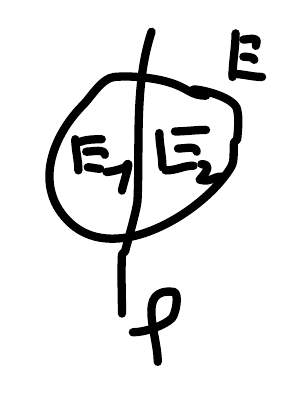
\begin{tikzpicture}[x=0.75pt,y=0.75pt,yscale=-0.75,xscale=0.75]
        %uncomment if require: \path (0,300); %set diagram left start at 0, and has height of 300
        
        %Shape: Free Drawing [id:dp7628728695496989] 
        \draw  [color={rgb, 255:red, 0; green, 0; blue, 0 }  ][line width=3] [line join = round][line cap = round] (146.33,63.67) .. controls (136.73,63.67) and (135.51,59.39) .. (124.33,55.67) .. controls (113.51,52.06) and (98.23,50.72) .. (87.33,51.67) .. controls (79.49,52.35) and (72.38,64.62) .. (67.33,69.67) .. controls (47.68,89.32) and (34.42,122.83) .. (59.33,145.67) .. controls (89.45,173.27) and (145.78,137.25) .. (162.33,109.67) .. controls (165.06,105.12) and (163.56,98.3) .. (164.33,93.67) .. controls (164.49,92.74) and (166.24,92.61) .. (166.33,91.67) .. controls (166.93,85.36) and (167.63,78.87) .. (166.33,72.67) .. controls (164.68,64.75) and (143.8,59.67) .. (138.33,59.67) ;
        %Shape: Free Drawing [id:dp2860373614820697] 
        \draw  [color={rgb, 255:red, 0; green, 0; blue, 0 }  ][line width=3] [line join = round][line cap = round] (111.33,22.67) .. controls (100.18,56.13) and (103.91,94.37) .. (102.33,130.67) .. controls (102.08,136.41) and (95.91,157.36) .. (94.33,163.67) .. controls (94.1,164.58) and (92.38,164.73) .. (92.33,165.67) .. controls (91.7,178.32) and (92.33,191) .. (92.33,203.67) ;
        %Shape: Free Drawing [id:dp08947191931178611] 
        \draw  [color={rgb, 255:red, 0; green, 0; blue, 0 }  ][line width=3] [line join = round][line cap = round] (99.33,215.67) .. controls (107.27,215.67) and (119.57,211.43) .. (124.33,206.67) .. controls (126.86,204.14) and (129.54,190.09) .. (125.33,189.67) .. controls (101.17,187.25) and (115.33,216.77) .. (115.33,234.67) ;
        %Shape: Free Drawing [id:dp9334586901493984] 
        \draw  [color={rgb, 255:red, 0; green, 0; blue, 0 }  ][line width=3] [line join = round][line cap = round] (165.33,23.67) .. controls (165.33,32.82) and (163.33,42.46) .. (163.33,51.67) ;
        %Shape: Free Drawing [id:dp04768711693928851] 
        \draw  [color={rgb, 255:red, 0; green, 0; blue, 0 }  ][line width=3] [line join = round][line cap = round] (170.33,27.67) .. controls (173,27.67) and (175.95,26.47) .. (178.33,27.67) .. controls (179.53,28.26) and (178.33,30.33) .. (178.33,31.67) ;
        %Shape: Free Drawing [id:dp5274114829816234] 
        \draw  [color={rgb, 255:red, 0; green, 0; blue, 0 }  ][line width=3] [line join = round][line cap = round] (170.33,38.67) .. controls (171.8,38.67) and (177.33,38.74) .. (177.33,40.67) ;
        %Shape: Free Drawing [id:dp6570628135366894] 
        \draw  [color={rgb, 255:red, 0; green, 0; blue, 0 }  ][line width=3] [line join = round][line cap = round] (163.33,49.67) .. controls (169.95,49.67) and (176.03,51.67) .. (182.33,51.67) ;
        %Shape: Free Drawing [id:dp8681341271113268] 
        \draw  [color={rgb, 255:red, 0; green, 0; blue, 0 }  ][line width=3] [line join = round][line cap = round] (116.33,87.67) .. controls (116.33,94.92) and (118.33,102.33) .. (118.33,109.67) ;
        %Shape: Free Drawing [id:dp6050366900451063] 
        \draw  [color={rgb, 255:red, 0; green, 0; blue, 0 }  ][line width=3] [line join = round][line cap = round] (126.33,86.67) .. controls (133.01,86.67) and (139.66,85.67) .. (146.33,85.67) ;
        %Shape: Free Drawing [id:dp7624577504469063] 
        \draw  [color={rgb, 255:red, 0; green, 0; blue, 0 }  ][line width=3] [line join = round][line cap = round] (128.33,97.67) .. controls (132.39,97.67) and (140.33,95.61) .. (140.33,99.67) ;
        %Shape: Free Drawing [id:dp6175909634779915] 
        \draw  [color={rgb, 255:red, 0; green, 0; blue, 0 }  ][line width=3] [line join = round][line cap = round] (120.33,111.67) .. controls (128.09,111.67) and (131.2,108.67) .. (138.33,108.67) ;
        %Shape: Free Drawing [id:dp110598214336876] 
        \draw  [color={rgb, 255:red, 0; green, 0; blue, 0 }  ][line width=3] [line join = round][line cap = round] (143.33,107.67) .. controls (152.66,107.67) and (142.07,117.6) .. (142.33,117.67) .. controls (150.18,119.63) and (150.17,115.67) .. (156.33,115.67) ;
        %Shape: Free Drawing [id:dp36668561089277496] 
        \draw  [color={rgb, 255:red, 0; green, 0; blue, 0 }  ][line width=3] [line join = round][line cap = round] (62.33,91.67) .. controls (62.33,98.21) and (64.33,104.94) .. (64.33,111.67) ;
        %Shape: Free Drawing [id:dp2428588068124462] 
        \draw  [color={rgb, 255:red, 0; green, 0; blue, 0 }  ][line width=3] [line join = round][line cap = round] (64.33,93.67) .. controls (69.02,91.79) and (74.29,91.67) .. (79.33,91.67) ;
        %Shape: Free Drawing [id:dp21516400666861557] 
        \draw  [color={rgb, 255:red, 0; green, 0; blue, 0 }  ][line width=3] [line join = round][line cap = round] (69.33,99.67) .. controls (73.39,99.67) and (81.33,97.61) .. (81.33,101.67) ;
        %Shape: Free Drawing [id:dp3834606938145779] 
        \draw  [color={rgb, 255:red, 0; green, 0; blue, 0 }  ][line width=3] [line join = round][line cap = round] (70.33,109.67) .. controls (73.02,109.67) and (75.65,110.67) .. (78.33,110.67) ;
        %Shape: Free Drawing [id:dp5890643945584151] 
        \draw  [color={rgb, 255:red, 0; green, 0; blue, 0 }  ][line width=3] [line join = round][line cap = round] (82.33,112.67) .. controls (85.3,112.67) and (92,110.83) .. (94.33,109.67) .. controls (95.18,109.25) and (95.91,106.82) .. (96.33,107.67) .. controls (96.99,108.98) and (92.33,123.09) .. (92.33,124.67) ;
    
        \end{tikzpicture}

        \item Псевдоплощадь существует, но не единственна.
    \end{enumerate}
\end{remark}

\begin{example}
    $E \in F$ \\
    $P_j$ это прямоугольник со сторонами параллельными осям координат, но произвольных размеров.
    \begin{enumerate}
        \item $\sigma_1(E) = \inf \left\{ \sum \sigma_1(P_j) \mid E \subset \bigcup\limits_{j=1}^N P_j \right\}$
        \item $\sigma_2(E) = \inf \left\{ \sum \sigma_2(P_j) \mid E \subset \bigcup\limits_{j=1}^\infty P_j \right\}$
    \end{enumerate}
    \begin{remark}
        $\sigma_1(E) \geq \sigma_2(E)$ и если $K = ([0, 1] \cap \Q) \times [0, 1] \Rightarrow \sigma_1(K) = 1, \sigma_2(K) = 0$
    \end{remark}
\end{example}

\begin{theorem}
    $\sigma_1$ -- псевдоплощадь. 
\end{theorem}

\begin{proof}
    \begin{enumerate}
        \item Если прямоугольник покрыть конечным числом прямоугольников, то у покрытия сумма площадей не меньше площади прямоугольника.
        (Т.к. можно провести все вертикальные и горизонтальные линии и разбить на дизъюнктивное объединение)

        \item 
        $\sigma_1(E) \stackrel{?}{=} \sigma_1(E_-) + \sigma_1(E_+)$ \\
        \circled{$\geq$} $E \subset P_1 \cup \ldots \cup P_n$,  $P_j = P_j^- \cup P_j^+$,  $\sigma_1(P_j) = \sigma_1(P_j^-) + \sigma_1(P_j^+)$ \\
        Тогда $\sum\limits_{j=1}^N \sigma_1(P_j) = \sum\limits_{j=1}^n \sigma_1(P_j^-) + \sum\limits_{j=1}^n \sigma_1(P_j^+) \geq \sigma_1(E_-) + \sigma_1(E_+)$ \\
        $\Rightarrow \sigma_1(E) \geq \sigma_1(E_-) + \sigma_1(E_+)$ \\
        
        \circled{$\leq$} $P_1, \ldots, P_k$ - покрытие $E_-$ с точность $\varepsilon$,  \\
        $P_{k + 1}, \ldots, P_n$ - покрытие $E_+$ с точность $\varepsilon$ \\
        $\Rightarrow \sigma_1(E_-) + \varepsilon \geq \sigma_1(P_1) + \ldots + \sigma_1(P_k)$ \\
        $\sigma_1(E_+) + \varepsilon \geq \sigma_1(P_{k + 1}) + \ldots + \sigma_1(P_n)$ \\
        $\Rightarrow \sigma_1(E_-) + \sigma_1(E_+) + 2\varepsilon \geq \sum\limits_{j = 1}^N \sigma_1(P_j) \geq \sigma_1(E)$

        \item Покрытие большего является покрытием меньшего.
        
         
    \end{enumerate}
\end{proof}

\begin{theorem}
    Псевдоплощадь $\sigma_1$ инварианта относительно сдвигов.
\end{theorem}

\begin{proof}
    Покрытие также сдвинется.
\end{proof}

\begin{remark}
    Проверить то же самое для $\sigma_2$.
\end{remark}



 \newpage

\subsection{Определенный интеграл.}

Считаем, что зафиксирована псевдоплощадь $\sigma$.


\begin{definition}
    $a \in \R \Rightarrow a_+ = \max(a, 0), a_- = \max(-a, 0)$ \\
    $a_+ + a_- = |a|, a_+ - a_- = a$ \\
    Аналогично для функции $f$. \\




    \tikzset{every picture/.style={line width=0.75pt}} %set default line width to 0.75pt        

    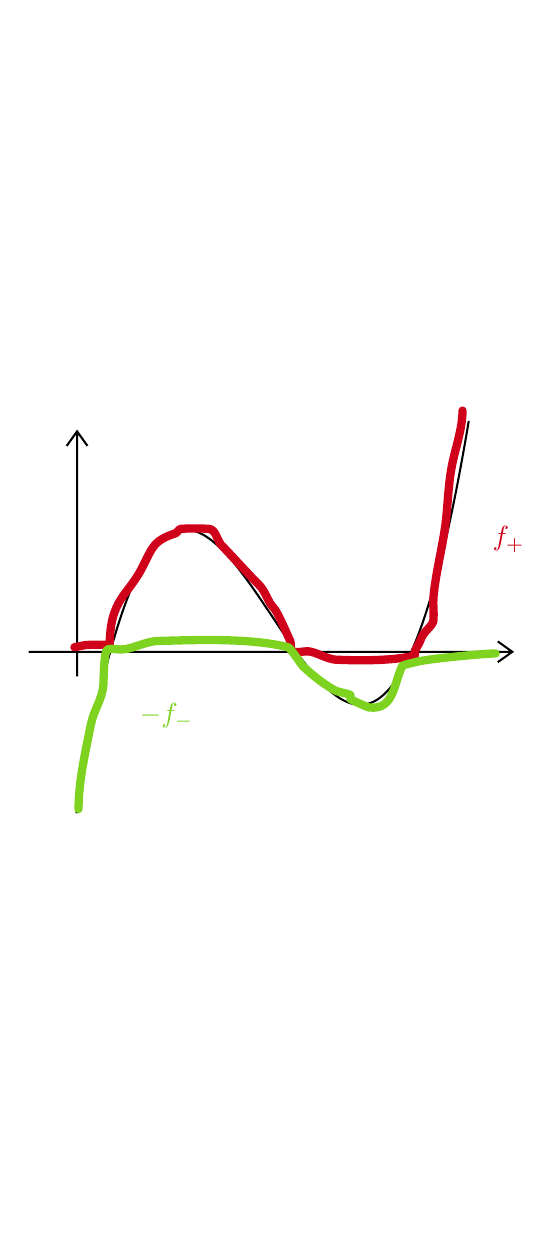
\begin{tikzpicture}[x=0.75pt,y=0.75pt,yscale=-1,xscale=1]
    %uncomment if require: \path (0,300); %set diagram left start at 0, and has height of 300
    
    %Shape: Axis 2D [id:dp9687964262664879] 
    \draw  (49,178.2) -- (282,178.2)(72.3,72) -- (72.3,190) (275,173.2) -- (282,178.2) -- (275,183.2) (67.3,79) -- (72.3,72) -- (77.3,79)  ;
    %Shape: Polynomial [id:dp4403110859007735] 
    \draw   (72,256) .. controls (135,-122) and (198,445) .. (261,67) ;
    %Shape: Free Drawing [id:dp20028065075963364] 
    \draw  [color={rgb, 255:red, 208; green, 2; blue, 27 }  ,draw opacity=1 ][line width=3] [line join = round][line cap = round] (71,176) .. controls (72.7,176) and (74.31,175.13) .. (76,175) .. controls (79.99,174.69) and (84.01,174.67) .. (88,175) .. controls (88.33,175.03) and (88,176.33) .. (88,176) .. controls (88,152.33) and (96.57,151.87) .. (104,137) .. controls (109.08,126.85) and (109.49,124.5) .. (120,121) .. controls (120.89,120.7) and (121.06,119.07) .. (122,119) .. controls (126.65,118.67) and (131.35,118.67) .. (136,119) .. controls (139.06,119.22) and (139.88,124.88) .. (142,127) .. controls (146.11,131.11) and (154.5,140.5) .. (160,146) .. controls (163.18,149.18) and (164.22,154.22) .. (167,157) .. controls (169.04,159.04) and (174.25,171.5) .. (175,173) .. controls (175.76,174.52) and (174.41,177.4) .. (176,178) .. controls (178.5,178.94) and (181.35,177.71) .. (184,178) .. controls (187.61,178.4) and (192.9,181.82) .. (197,182) .. controls (207.43,182.45) and (224.21,182.7) .. (235,180) .. controls (235.65,179.84) and (234.74,178.61) .. (235,178) .. controls (235.88,175.94) and (237.29,174.12) .. (238,172) .. controls (239.23,168.3) and (243.75,165.79) .. (244,163) .. controls (244.33,159.35) and (243.7,155.65) .. (244,152) .. controls (244.98,140.24) and (248.71,126.65) .. (250,115) .. controls (251.01,105.93) and (251.22,96.88) .. (253,88) .. controls (254.57,80.14) and (258,70.59) .. (258,62) ;
    %Shape: Free Drawing [id:dp9900303760322543] 
    \draw  [color={rgb, 255:red, 126; green, 211; blue, 33 }  ,draw opacity=1 ][line width=3] [line join = round][line cap = round] (73,254) .. controls (73,240.57) and (76.39,226.03) .. (79,213) .. controls (80.4,205.98) and (84.31,201.58) .. (85,194) .. controls (85.08,193.17) and (85.12,177.47) .. (87,177) .. controls (89.59,176.35) and (92.36,177.38) .. (95,177) .. controls (100,176.29) and (106.02,173.13) .. (111,173) .. controls (129.51,172.51) and (155.69,171.42) .. (174,176) .. controls (175.04,176.26) and (180.25,184.25) .. (181,185) .. controls (184.41,188.41) and (191.44,194.22) .. (197,197) .. controls (198.69,197.84) and (202.69,198.13) .. (204,199) .. controls (204.55,199.37) and (203.45,200.63) .. (204,201) .. controls (204.77,201.51) and (212.01,204.88) .. (213,205) .. controls (225.08,206.51) and (224.79,193.42) .. (229,185) .. controls (229.26,184.49) and (234.93,183.36) .. (236,183) .. controls (239.23,181.92) and (267.64,179) .. (274,179) ;
    
    % Text Node
    \draw (271,116.4) node [anchor=north west][inner sep=0.75pt]  [color={rgb, 255:red, 208; green, 2; blue, 27 }  ,opacity=1 ]  {$f_{+}$};
    % Text Node
    \draw (101,201.4) node [anchor=north west][inner sep=0.75pt]  [color={rgb, 255:red, 126; green, 211; blue, 33 }  ,opacity=1 ]  {$-f_{-}$};
\end{tikzpicture}

    $\Gamma_f = \left\{(x, f(x)) \in \R^2\right\}$ \\
    Для $f \geq 0 \  P_f = \left\{ (x, y) : y \in [0, f(x)]\right\}$ - подграфик f. \\
    Для $f \geq 0$ на $[a, b], P_f[a, b] = \left\{ (x, y) : x \in [a, b], y \in [0, f(x)]\right\}$ - подграфик f.
\end{definition}

\begin{remark}
    $f$ - непр $\Rightarrow f_+, f_-$ - непр.
\end{remark}

\begin{definition}
    $f$ - непр. на $[a, b]$, тогда \\
    \[\int_a^b f(x) dx = \sigma(P_{f_+} [a, b]) - \sigma(P_{f_-}[a, b])\]
\end{definition}

\begin{properties}
    \item $\int_a^a f \ dx = 0$
    \item $\int_a^b 0 \  dx = 0$
    \item $f \geq 0$ на $[a, b] \Rightarrow \int_a^b f \ dx \geq 0$
    \item $\int_a^b - f \ dx = -\int_a^b f \ dx$
    \item $\int_a^b c \ dx = c \cdot (b - a)$
    \item $f \geq 0$ на $[a, b] \wedge \int_a^b f \ dx = 0 \Rightarrow f = 0$ на $[a, b]$
    \begin{proof}
        Т.к. функция непрерывна, то если существует точка $f$ со значением не 0,
            то можно найти окрестность со значением $>$ 0 и там будет ненулевая площадь
    \end{proof}

    \item(Аддитивность интеграла) $c \in [a, b] \Rightarrow \int_a^b f dx = 
    \int_a^c f dx +\int_c^b f dx$
    
    \begin{proof}
        Следует из аддитивности псевдоплощади.
    \end{proof}

    \begin{remark}
        Соглашение: $\int_a^b f dx = - \int_b^a f dx \Rightarrow$ аддитивность верна и 
        для $c \not \in [a, b]$
    \end{remark}

    \item(Монотонность) $f \geq g$ на $[a ,b] \Rightarrow \int_a^b f dx \geq 
    \int_a^b g dx$
    
    \begin{proof}
        $f \geq g \Rightarrow f_+ \geq g_+ \wedge f_- \leq g_-$
    \end{proof}

    \item $(b - a) \min\limits_{[a, b]} f \leq \int_a^b f dx \leq (b - a) \max\limits_{[a, b]} f$
    \item(Теорема о среднем) $\exists c \in [a, b] : \int_a^b f dx = f(c) \cdot (b-a)$
    \begin{proof}
    \[\frac {\int_a^b f dx} {b - a} \in [\min f, \max f] \Rightarrow \exists c\]
    \end{proof}

    \item(Теорема Барроу) $\Phi(x) = \int_a^x f(t) dt, \Psi(x) = \int_x^b f(t) dt$ \\
    $\Phi$ - интеграл с переменным верхним пределом, $\Psi$ - нижним \\
    $\Phi' = f, \Psi' = -f$
    \begin{proof}
        $x_1, x_2$ 
        \[\frac {\Phi(x_1) - \Phi(x_2)} {x_1 - x_2}
        = \frac {\int_{x_2}^{x_1} f(t) dt} {x_1 - x_2}  
        \stackrel{x_1- fix}{\Rightarrow} \lim_{x_2 \to x_1} \frac {\Phi(x_1) - \Phi(x_2)} {x_1 - x_2}
        = \lim_{x_2 \to x_1} \frac {\int_{x_2}^{x_1} f(t) dt} {x_1 - x_2}
        = \lim_{x_2 \to x_1} f(\theta)\] \\
        где $\theta$ лежит между $x_1$ и $x_2$ \\
        $\Rightarrow \Phi'(x_1) = f(x_1)$ \\
        $\Phi + \Psi = const \Rightarrow \Psi' = -f$
    \end{proof}

    \item(формула Ньютона-Лейбница) $F$ - первообразная $\Rightarrow$ \\
    $\int_a^b f(x) dx = F(b) - F(a) = F|_a^b$
    \begin{proof}
        \[ \Phi(x) = \int_a^x f \Rightarrow F = \Phi + c \Rightarrow F(b) - F(a)
        = \Phi(b) - \Phi(a) = \int_a^b f \]
    \end{proof}

    \item(Линейность интеграла) \[f, g \in C[a, b], \alpha, \beta \in R \Rightarrow
    \int_a^b (\alpha f + \beta g) dx = \alpha \int_a^b f dx + \beta \int_a^b g dx \] 
    \begin{proof}
        Следует из существования первообразной.
    \end{proof}
    \item $|\int_a^b f dx| \leq \int_a^b |f| dx$
    \begin{proof}
        \[ \left|\int_a^b f\right| = \left|\int_a^b f_+ - \int_a^b f_-\right| \leq
            \int_a^b f_+ + \int_a^b f_- = \int_a^b |f| \]
    \end{proof}
    
    \item(формула интегрирования по частям)
    \[f, g \in C^1[a, b] \Rightarrow
    \int_a^b f(x) g'(x) dx = f(x)g(x)\bigg|_a^b - \int_a^b f'(x)g(x) dx \]

    \begin{proof}
        Следует из формулы Ньютона-Лейбница и формулы интегрирования по частям для неопределенного интеграла.
    \end{proof}

    \item(Замена переменной) $ f:[a, b] \to \R, \phi : [c, d] \to [a, b], \phi \in C^1[c, d]$ 
    \[\Rightarrow
    \forall p, q \in [c, d] \hence \int_p^q f(\phi(t)) \phi'(t) dt
    = \int_{\phi(t)}^{\phi(q)} f(x) dx\]

    \begin{example}
        \begin{enumerate}
            \item \[ \int_0^1 e^{\sin(x)} \cos(x) \ dx = [\sin(x) = y, dy = \cos(x) dx] 
            = \int_{\sin(0)}^{sin(1)} e^y \ dy = \ldots \]
            \item \[ \int_0^1 \sqrt{1 - x^2} \ dx = [x = \sin(y), dx 
            = \cos(y) dy] = \int_0^{\arcsin(1)} \sqrt{1 - \sin^2(y)} \cos(y) \ dy 
            = \int_0^{\frac \pi 2} \cos^2(y) \ dy \] 
            \[ = \int_0^{\frac \pi 2} \frac {1 + \cos^2(y)} 2 \ dy
            = \int_0^{\frac \pi 2} \frac 1 2 \ dy = \frac \pi 4\]
        \end{enumerate}
    \end{example}
\end{properties}
